\chapter{Methodology Part 1: Geometry Representation and Point Placement}

In this section, we will talk about the initial import of surface triangulation and storing the surface as a collection of bezier surface patches. Then, the point placement subroutine is explained which decides the mesh element structure. Lastly, a small discussion on the local mesh element quality improvement is added to explain the face swapping algorithm. 

\section{Surface Import}

\subsection{Surface Representation - A brief overview}

Surfaces can be represented in various forms. A surface could be represented by an explicit equation such as the one shown below.

\begin{equation}
z = F(x,y)
\end{equation}

Where the coordinate $z$ can be found by solving the aforementioned explicit equation, given the remaining two coordinates $x$ and $y$.  Explicit form of surfaces are easy to trace. However, it is not very versatile. Surfaces could also be represented with their implicit form, given by an implicit equation such as the one shown below.

\begin{equation}
F(x, y, z) = 0
\end{equation}

Here, solutions to the implicit equation represent points on the three dimensional surface. Figure \ref{fig-imex} shows an implicit and an explicit surface together with their mathematical formulations.

\begin{figure}
  \begin{subfigure}{0.5\linewidth}
  \centering
  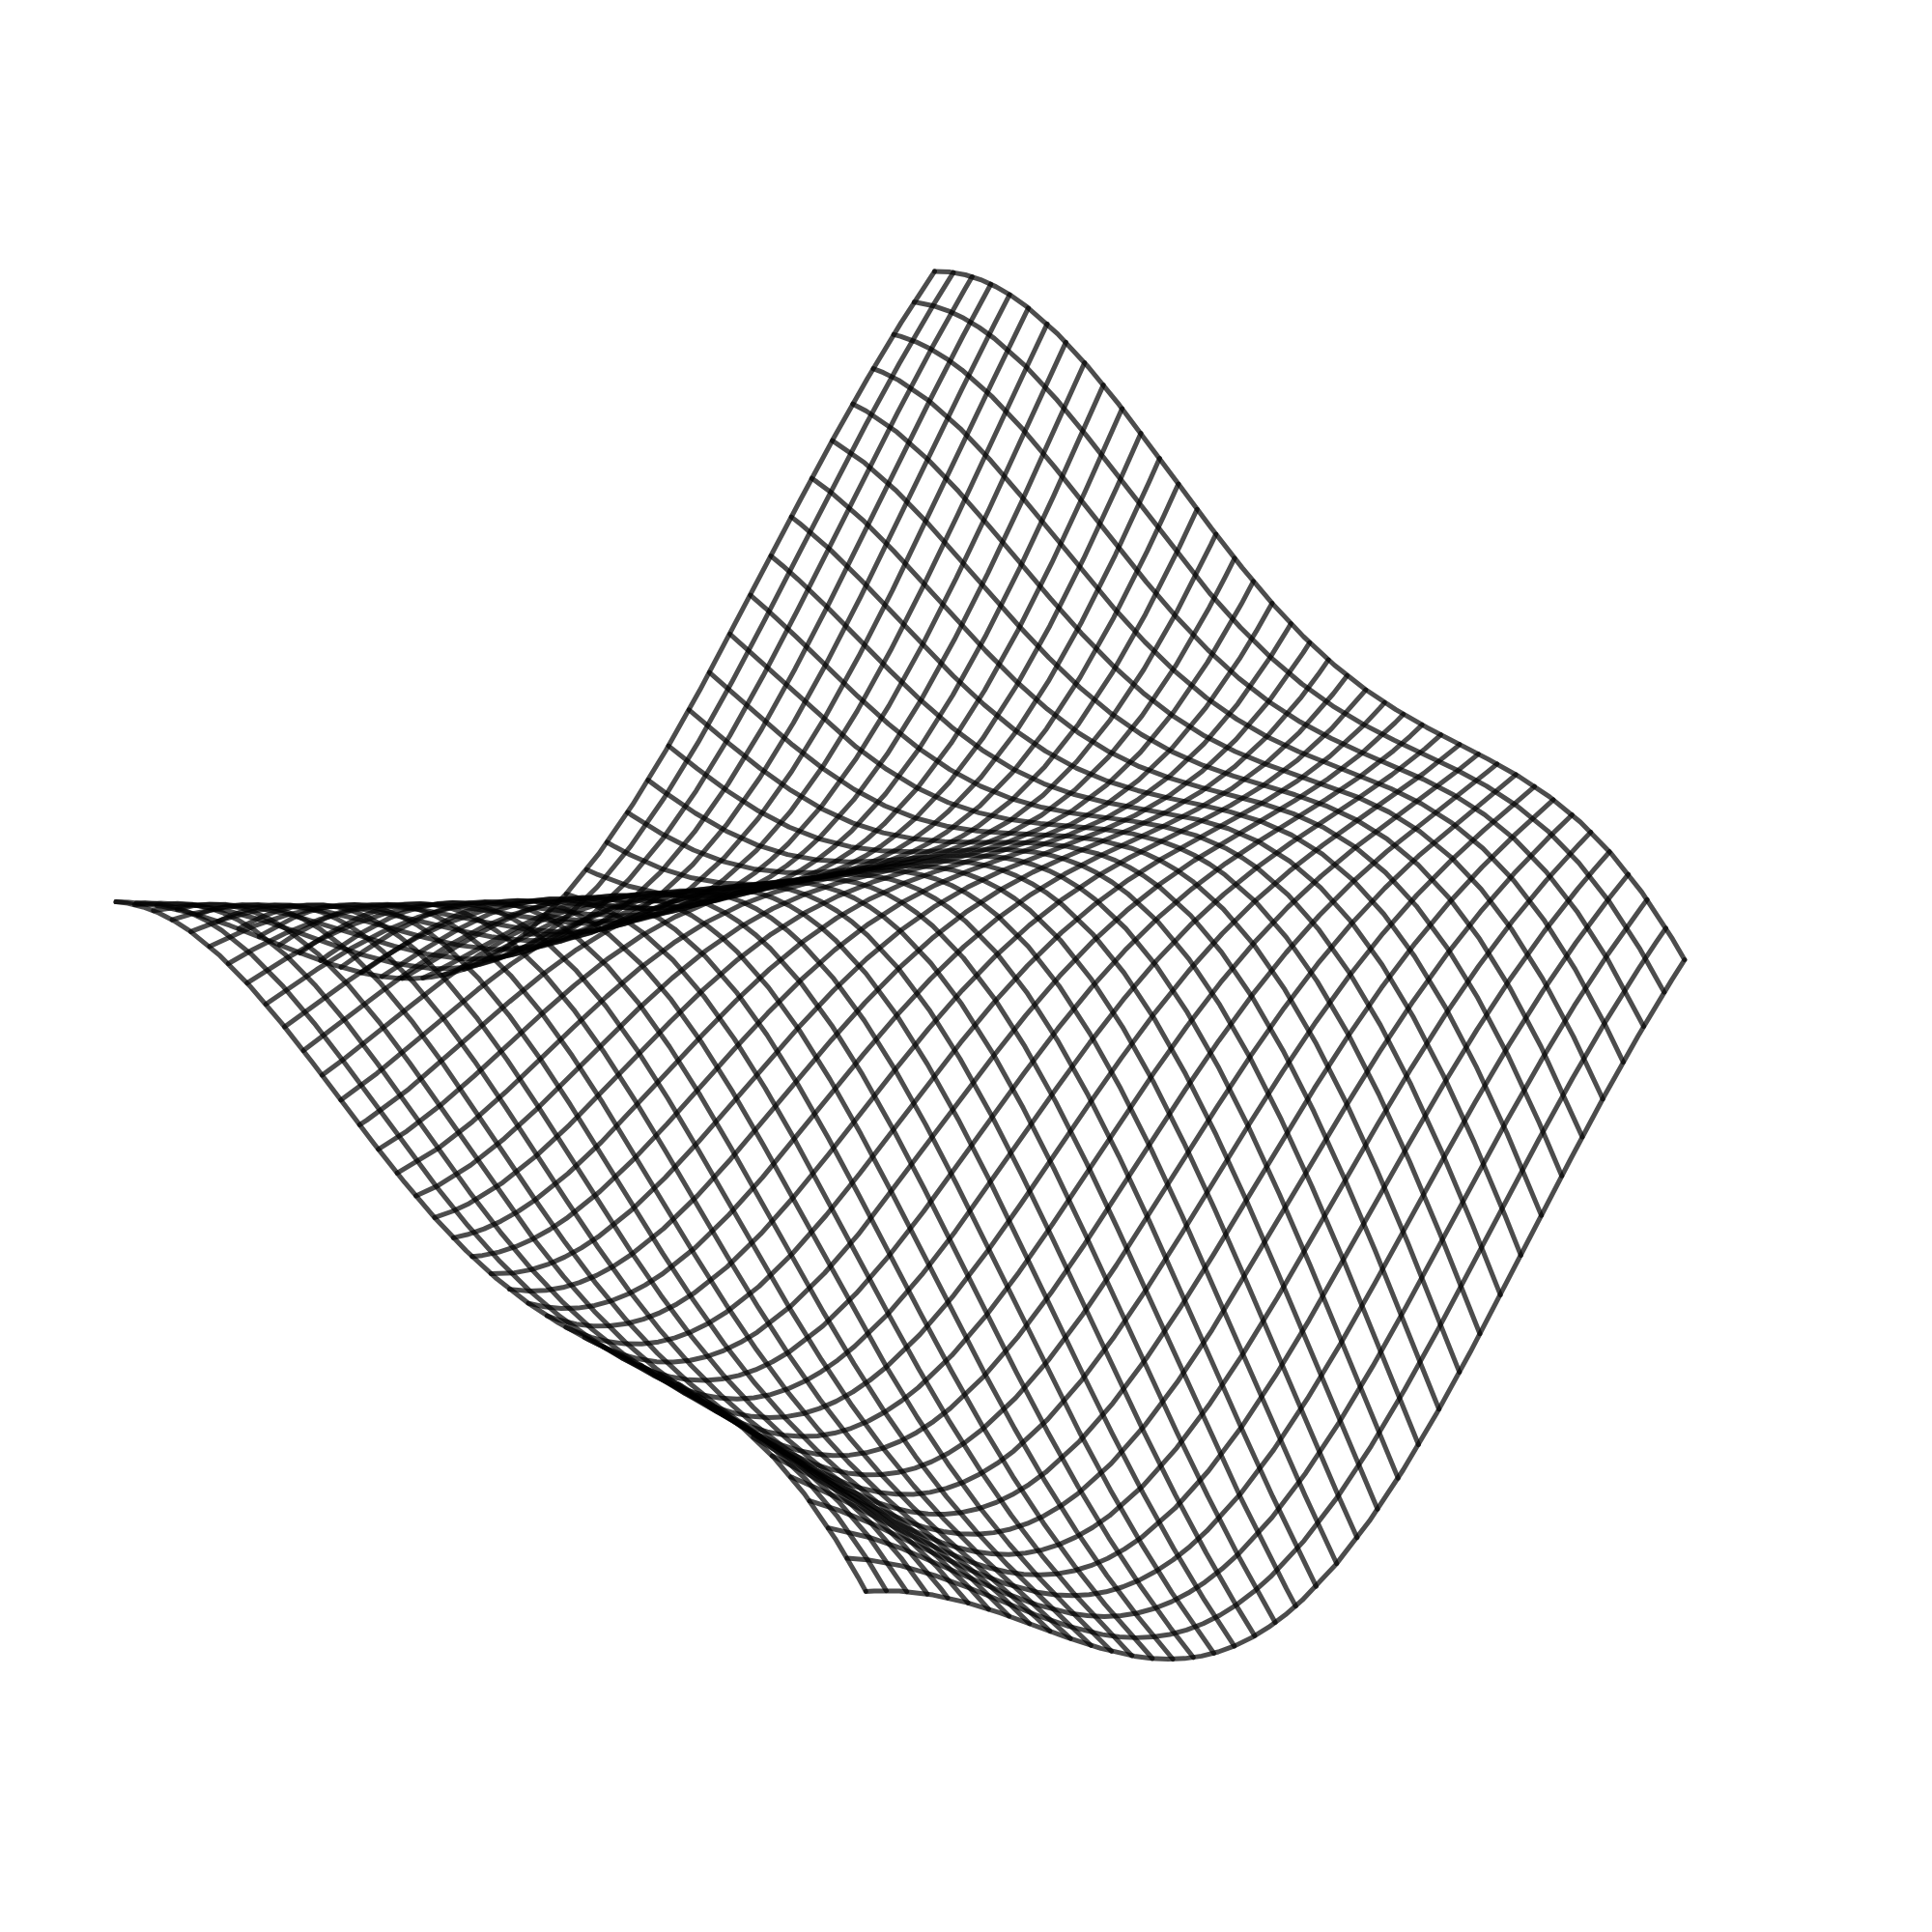
\includegraphics[width=0.9\linewidth]{img/m1/explicit.png}
  \caption{}
  \label{fig-explicit}
  \end{subfigure}
  \begin{subfigure}{0.5\linewidth}
    \centering
    
\includegraphics[width=0.8\linewidth]{img/m1/implicit.png}
    \caption{}
  \end{subfigure}
  \caption{(a) An explicit surface, given by $z = \cos ((x+y))+\frac{x^{2}}{6}-\frac{y^{2}}{6}$. (b) An implicit surface, given by $2 y\left(y^{2}-3 x^{2}\right)\left(1-z^{2}\right)+\left(x^{2}+y^{2}\right)^{2}-\left(9 z^{2}-1\right)\left(1-z^{2}\right)=0$. }
  \label{fig-imex}
\end{figure}

Apart from the explicit and implicit forms, surfaces can also be represented in their parametric form. The coordinates of a point $(x,y,z)$ of the surface patch are expressed as functions of parameters $u$ and $v$ in a closed rectangle:

\begin{equation}
x=x(u, v), \quad y=y(u, v), \quad z=z(u, v), \quad u_{1} \leq u \leq u_{2}, \quad v_{1} \leq v \leq v_{2}.
\end{equation}

In vector notation, the parametric surface can be specified by a vector-valued function

\begin{equation}
\mathbf{r}=\mathbf{r}(u, v)
\end{equation}

The parametric representation of surfaces is the most versatile out of the three. It is axis independent and is highly flexible in terms of defining complex intersections and point classification. It is generally easier to manipulate free-form shapes in parametric form than implicit or explicit forms  \cite{patrikalakis2009shape}. Hence, most of the CAD packages use parametric form of the surfaces to manipulate them. Bezier surface patch is one example of parametric form of a surface. 

\subsection{Surface File Format}


\begin{figure}
  \centering
  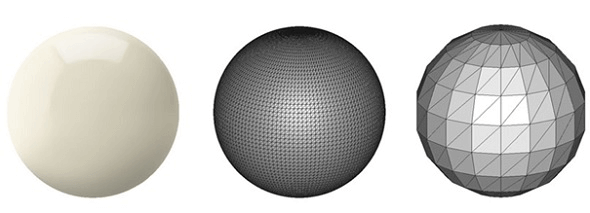
\includegraphics[width=\linewidth]{img/m1/tessellation.png}
  \caption{The perfect spherical surface on the left is approximated by tessellations. The figure on the right uses big triangles, resulting in a coarse model. The figure on the center uses smaller triangles and achieves a smoother approximation \cite{fileFormat}}
  \label{fig-tesellation}
\end{figure}

Given a free-form 3D surface geometry, various CAD packages could be used to encode it and store it in a file. Encoding the geometry using an approximate mesh is one of the most common methods adopted to store a surface geometry. An approximate mesh is created by covering the surface geometry with a series of tiny imaginary polygons. Trianlges are the most common polygon used for mesh generation. The encoded surface mesh can be stored in a file for sharing and future reference purposes. These files store the vertices of the triangles as well as the outward normal directions to the triangles. This process of tiling a surface with non-verlapping geometric shapes is also known as tessellation. Hence, the file formats used for storing the surface representation are called tessellated formats.

Due to the independent development of various CAD packages, a plethora of surface file formats are present in the mesh generation ecosystem. Many of these formats, such as DWG file format by AutoCAD and BLEND file format by Blender are proprietary. Hence, many of these cannot be shared between people working on different CAD packages. Native file formats are used to solve this problem. These formats can be shared easily among people working on different meshing softwares. One of the most common neutral surface file format is the STL (STereoLithography) file format. This format is compatible with most of the CAD and visualization softwares. Hence, we use the STL file format to import the surface geometry into our mesh generation algorithm.

An STL file stores the surface as a triangulated mesh. The following information is stored for all the triangles in teh STL file format:

\begin{enumerate}
  \item The coordinates of the vertices
  \item The components of the unit normal vector to the triangle pointing outwards with respect to the 3D model
\end{enumerate}

Innumerable software packages are available online which can be used to triangulate a surface (see \cite{meshSoftware} for a list of such softwares). A fine triangular mesh can be considered as an approximate encoding of a given surface geometry. The approximation could be improved by increasing the number of triangles or decreasing their size. However, using smaller triangles results in larger number of triangles needed to tile the surface. This increases the mesh file size. Hence, a user should define the mesh element size according to the kind of refinement needed.

\section{Surface Import and Segmentation using Common Geometry Module (CGM)}

As explained earlier, we import the surface geometry as a triangulation as an STL file. The Common Geometry Module (CGM) package is used to read the surface file and store the triangulation for further processing. The triangulated surface is stored as a collection of segmented sub-surfaces. The segmentation in CGM is done by identifying features in the surface. The only input parameter for surface segmentation accepted by CGM is the feature angle. We keep this feature angle value to be 135{$^\circ{}$}. This value helps us to identify sharp corners and edges on the surface. Figure \ref{fig-surfSegment} shows a surface triangulation of an arbitrary mechanical part. The surface triangulation is segmented into 10 sub-surfaces, which are identified by the sharp features on the surface. Four of these are shown in outline in the figure.

Each triangle imported in CGM is stored as a quartic-bezier patch. We will refer to the imported triangulation as $T$ and the underlying bezier surface representation as $S$. The underlying bezier surface representation $S$ is considered to be the ground truth for the surface and the mesh points are placed directly over $S$. Initial imported triangulation $T$ is taken as the initial mesh. We use a closed advancing layer mesh generation methodology. There are advantages and disadvantages of using such a methodology. Open advancing layer method requires less work overall to generate the mesh as there are no points to delete or reconnect to, ahead of the front. On the other hand, handling mesh layer collisions is  more tricky in open advancing layer method as no connectivity information is available ahead of the front in such methods. This leads to abrupt layer closures, which are undesirable in an anisotropic mesh.

Closed advancing layer mesh generation method generates a valid surface mesh at any point in the mesh generation process. Hence, there is more flexibility in terms of when to stop the marching layers and output the mesh in its current state. Additionally, connectivity information is known ahead of the front. This information is helpful while tackling layer collisions. This will be explained in more detail when we talk about handling front collisions in *ref*.

\begin{figure}
\centering
\begin{subfigure}{.5\textwidth}
  \centering
  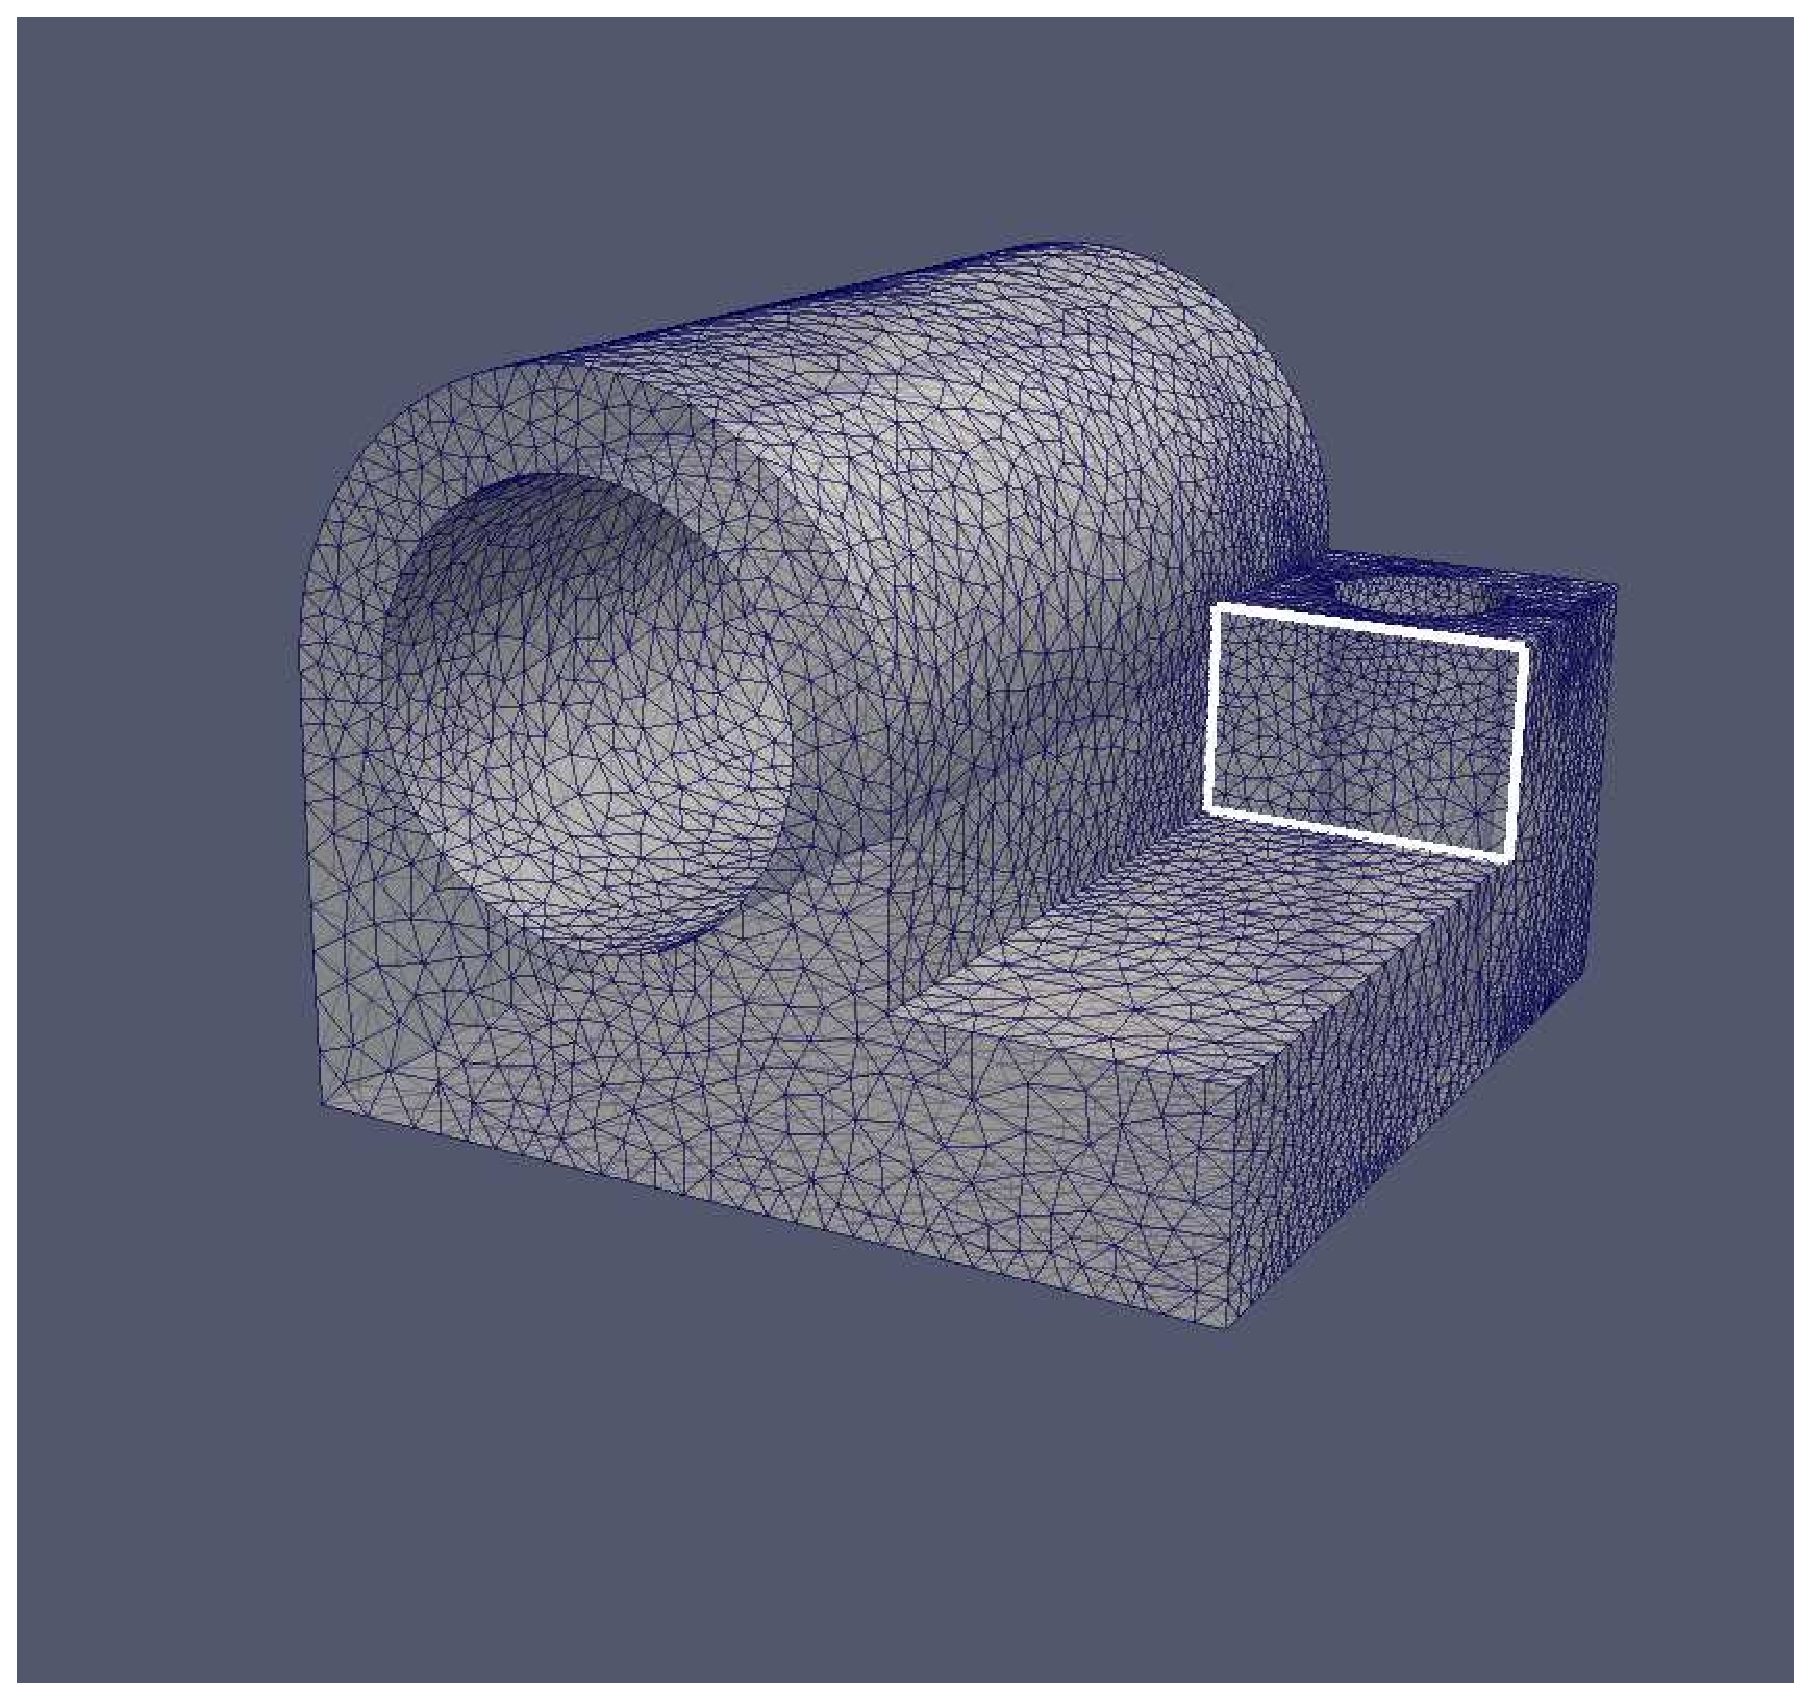
\includegraphics[width=.8\linewidth]{img/m1/surfSegmentation/surf0.eps}
  \caption{}
  \label{surf0}
\end{subfigure}%
\begin{subfigure}{.5\textwidth}
  \centering
  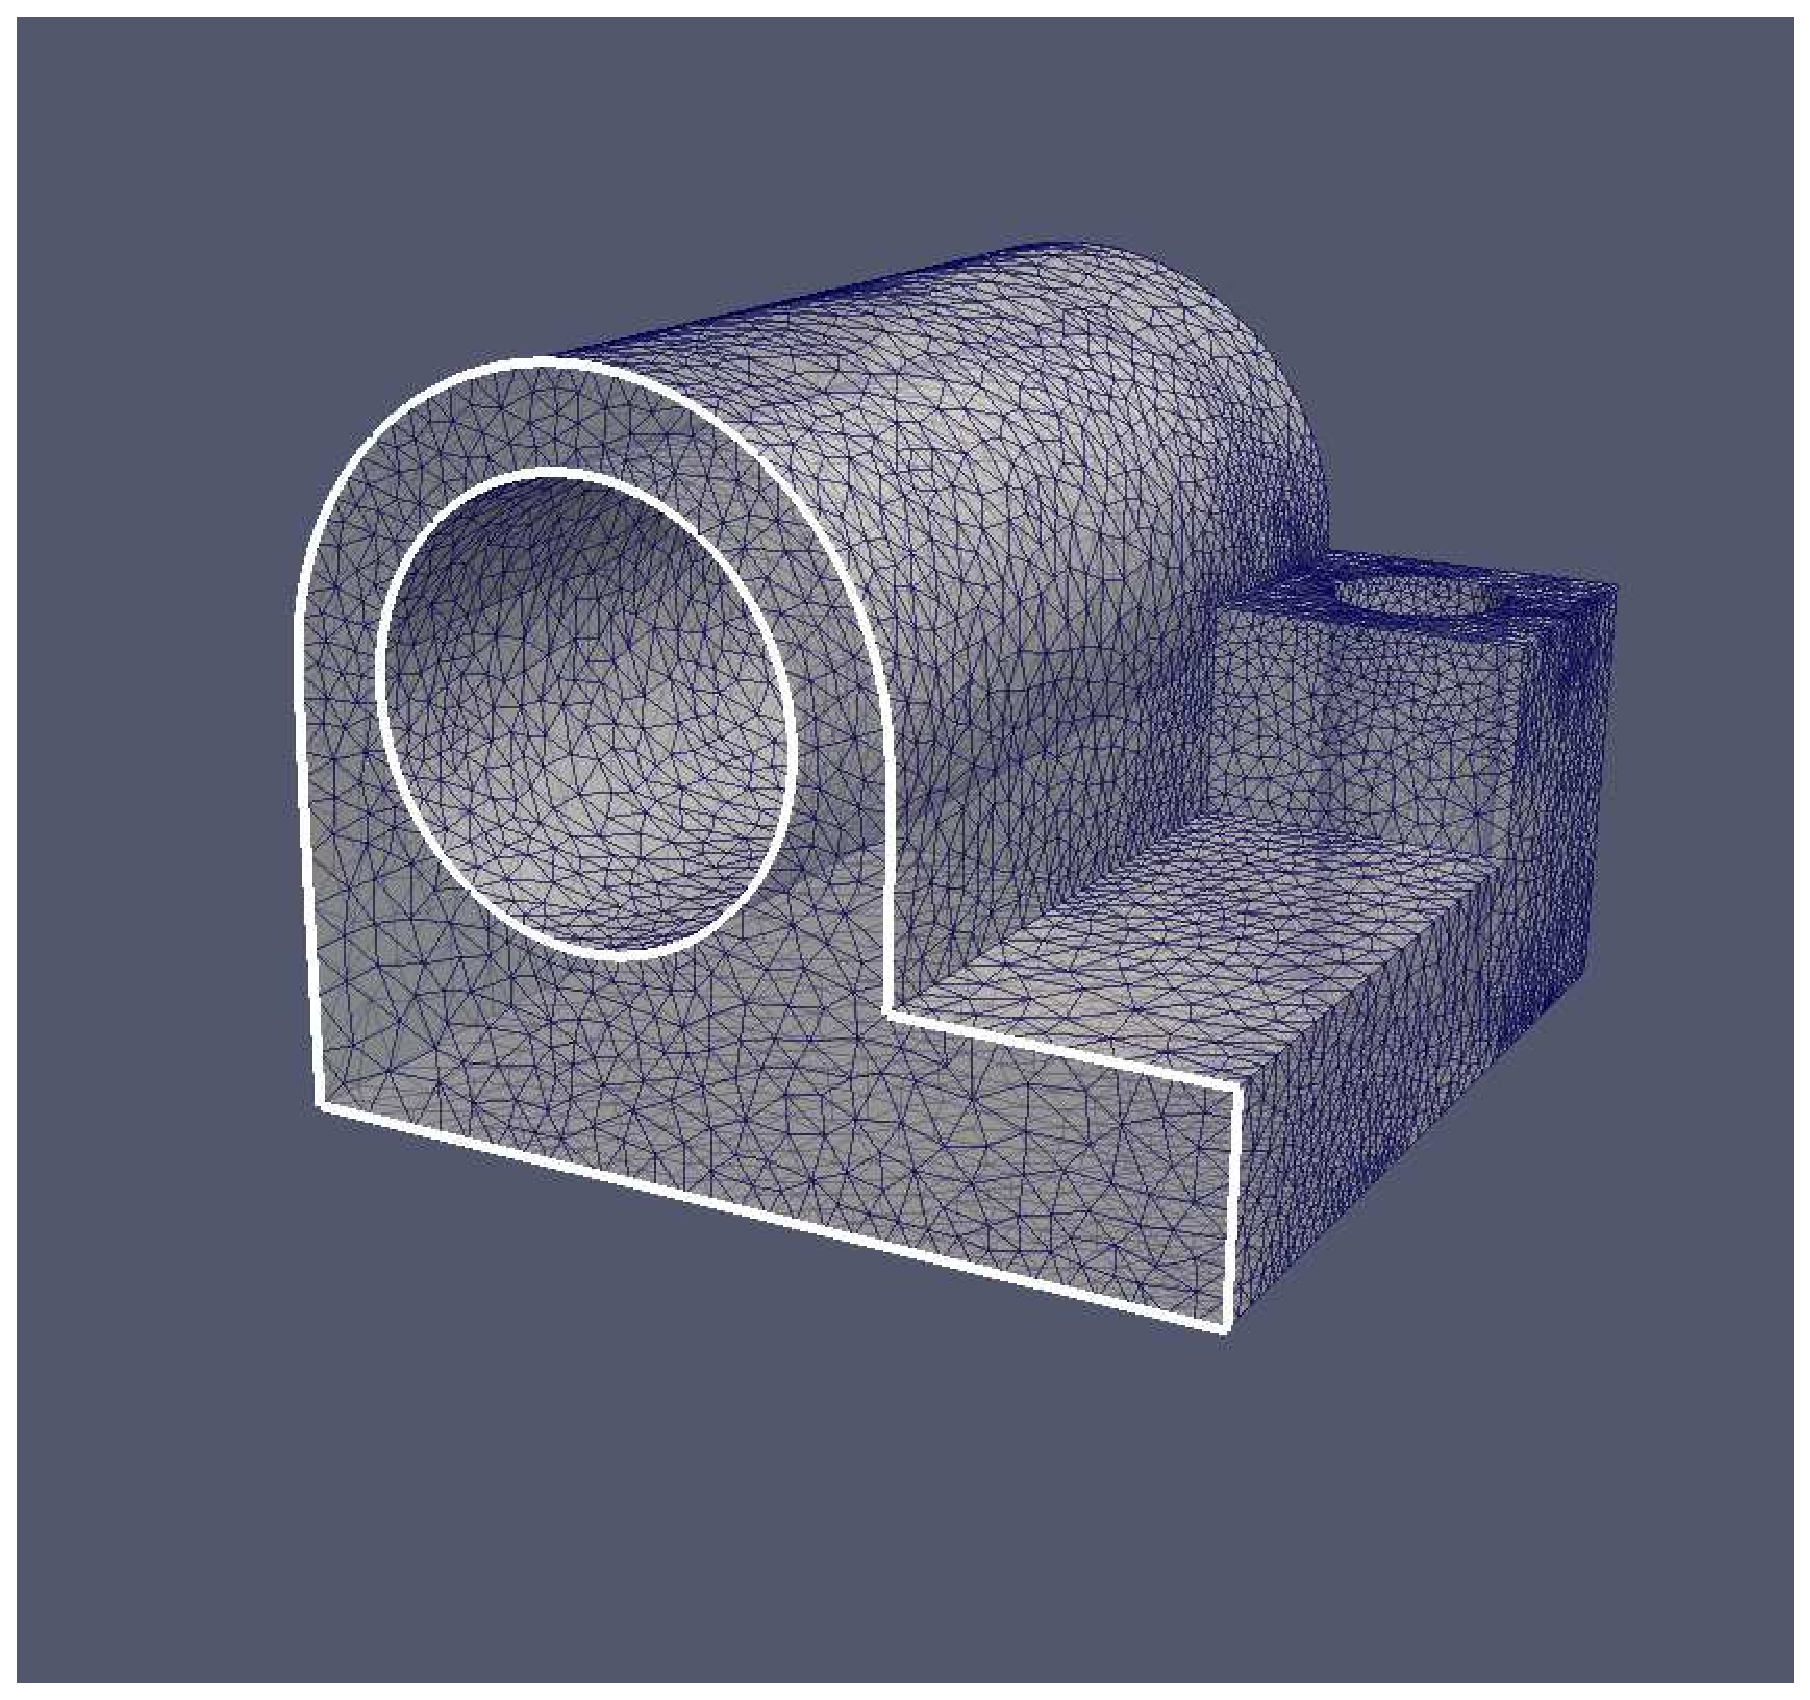
\includegraphics[width=.8\linewidth]{img/m1/surfSegmentation/surf3.eps}
  \caption{}
  \label{surf1}
\end{subfigure}
\begin{subfigure}{.5\textwidth}
  \centering
  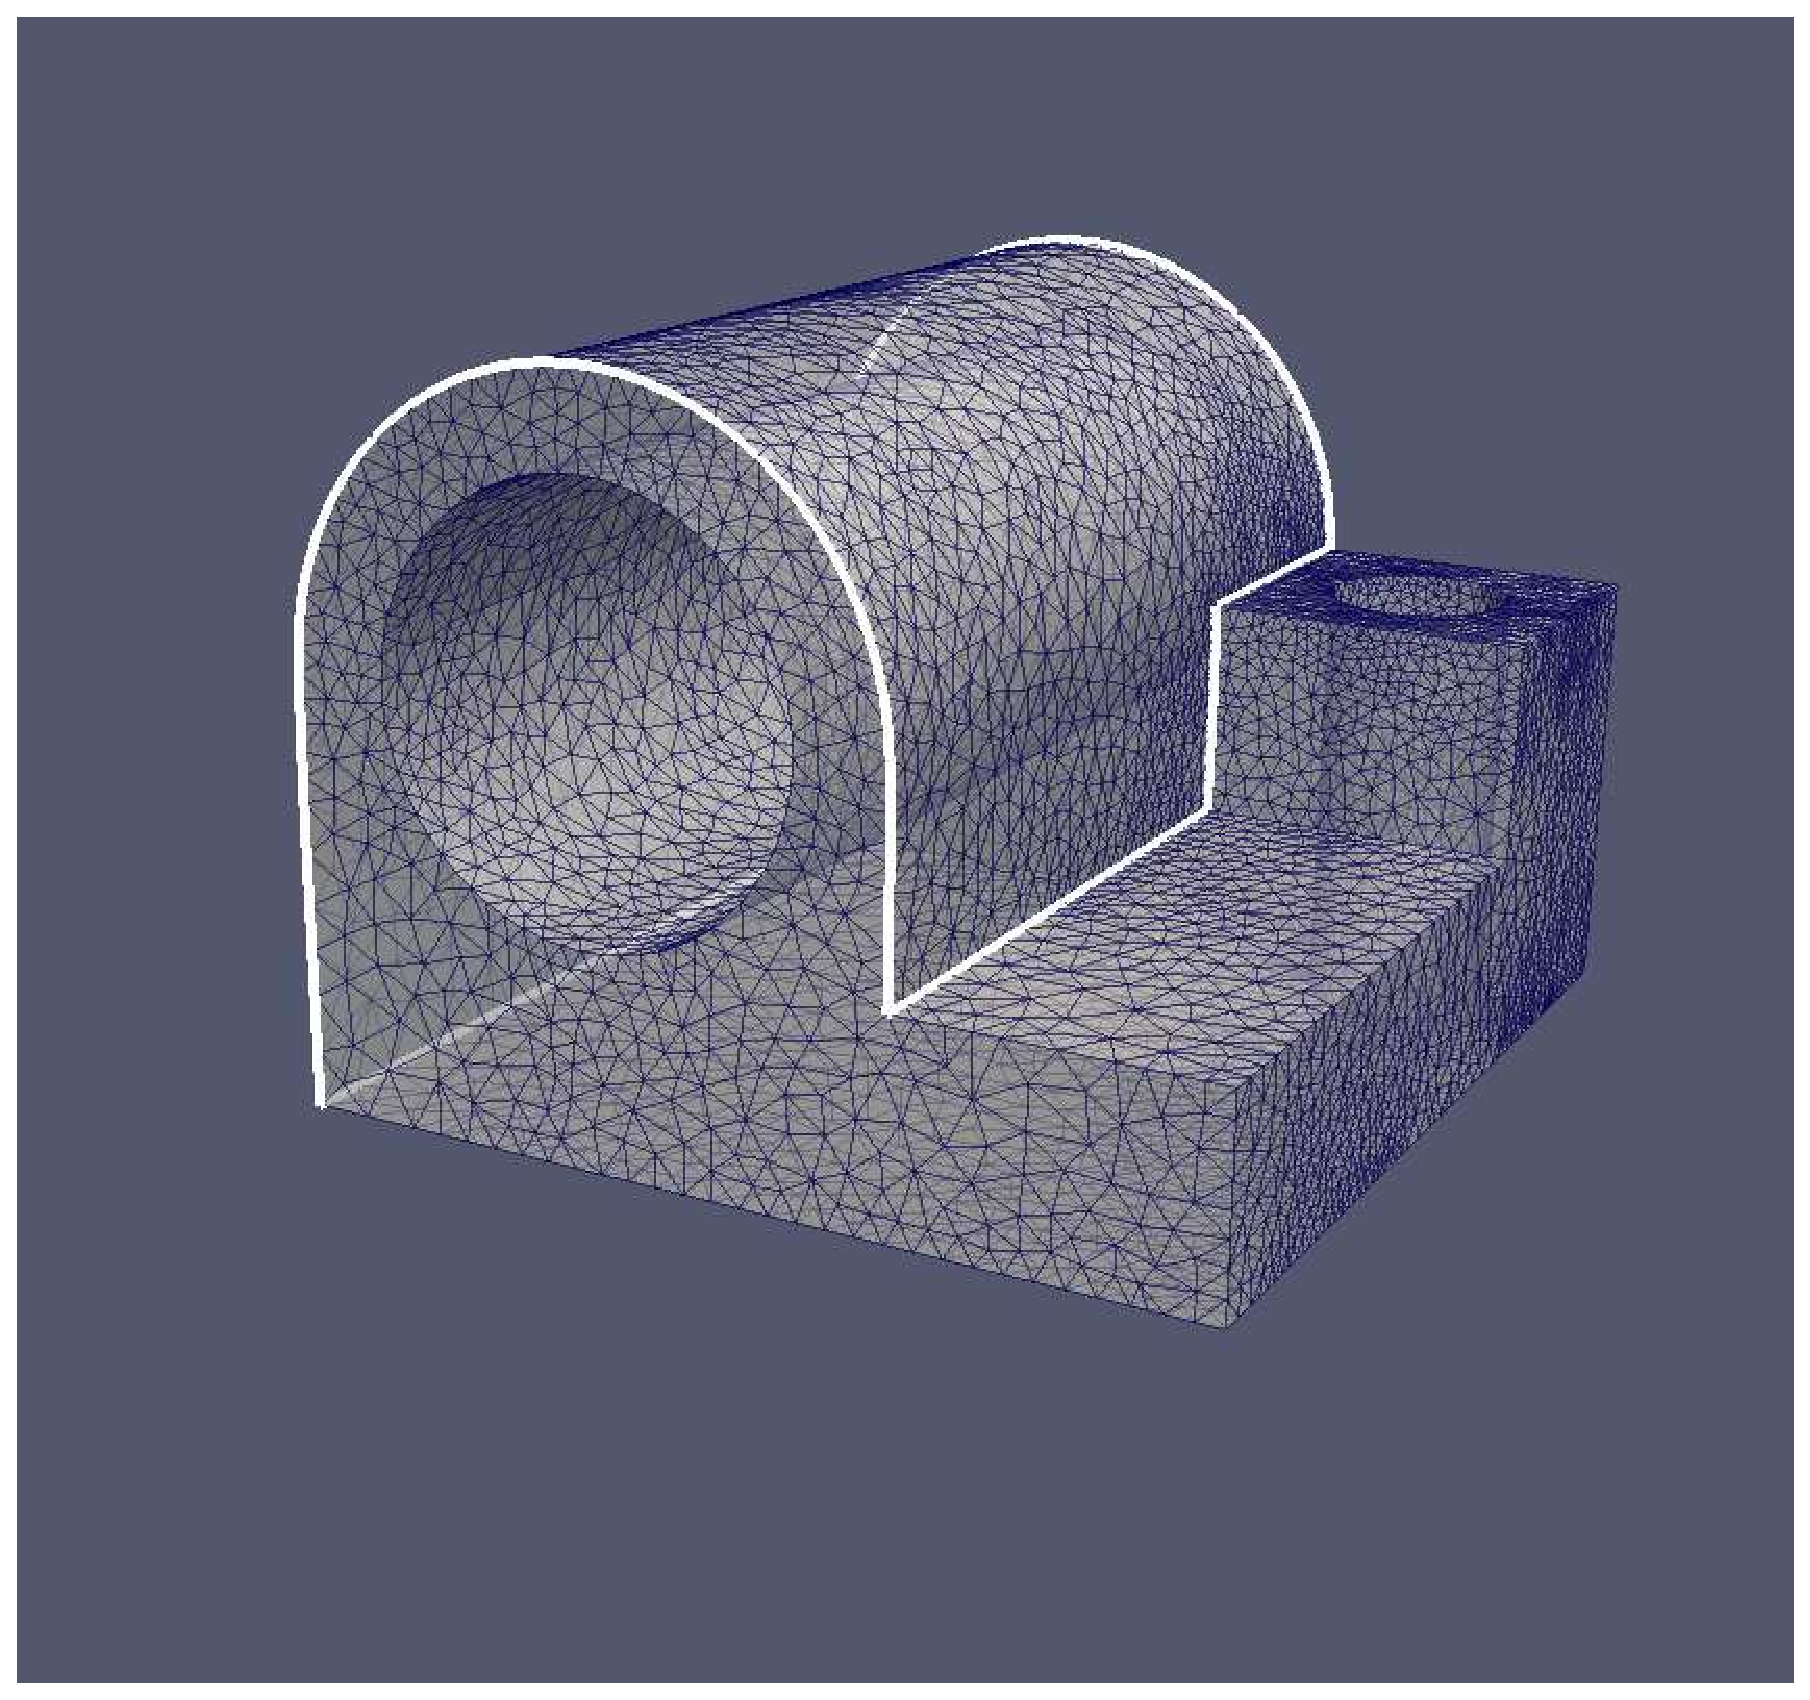
\includegraphics[width=.8\linewidth]{img/m1/surfSegmentation/surf5.eps}
  \caption{}
  \label{surf2}
\end{subfigure}%
\begin{subfigure}{.5\textwidth}
  \centering
  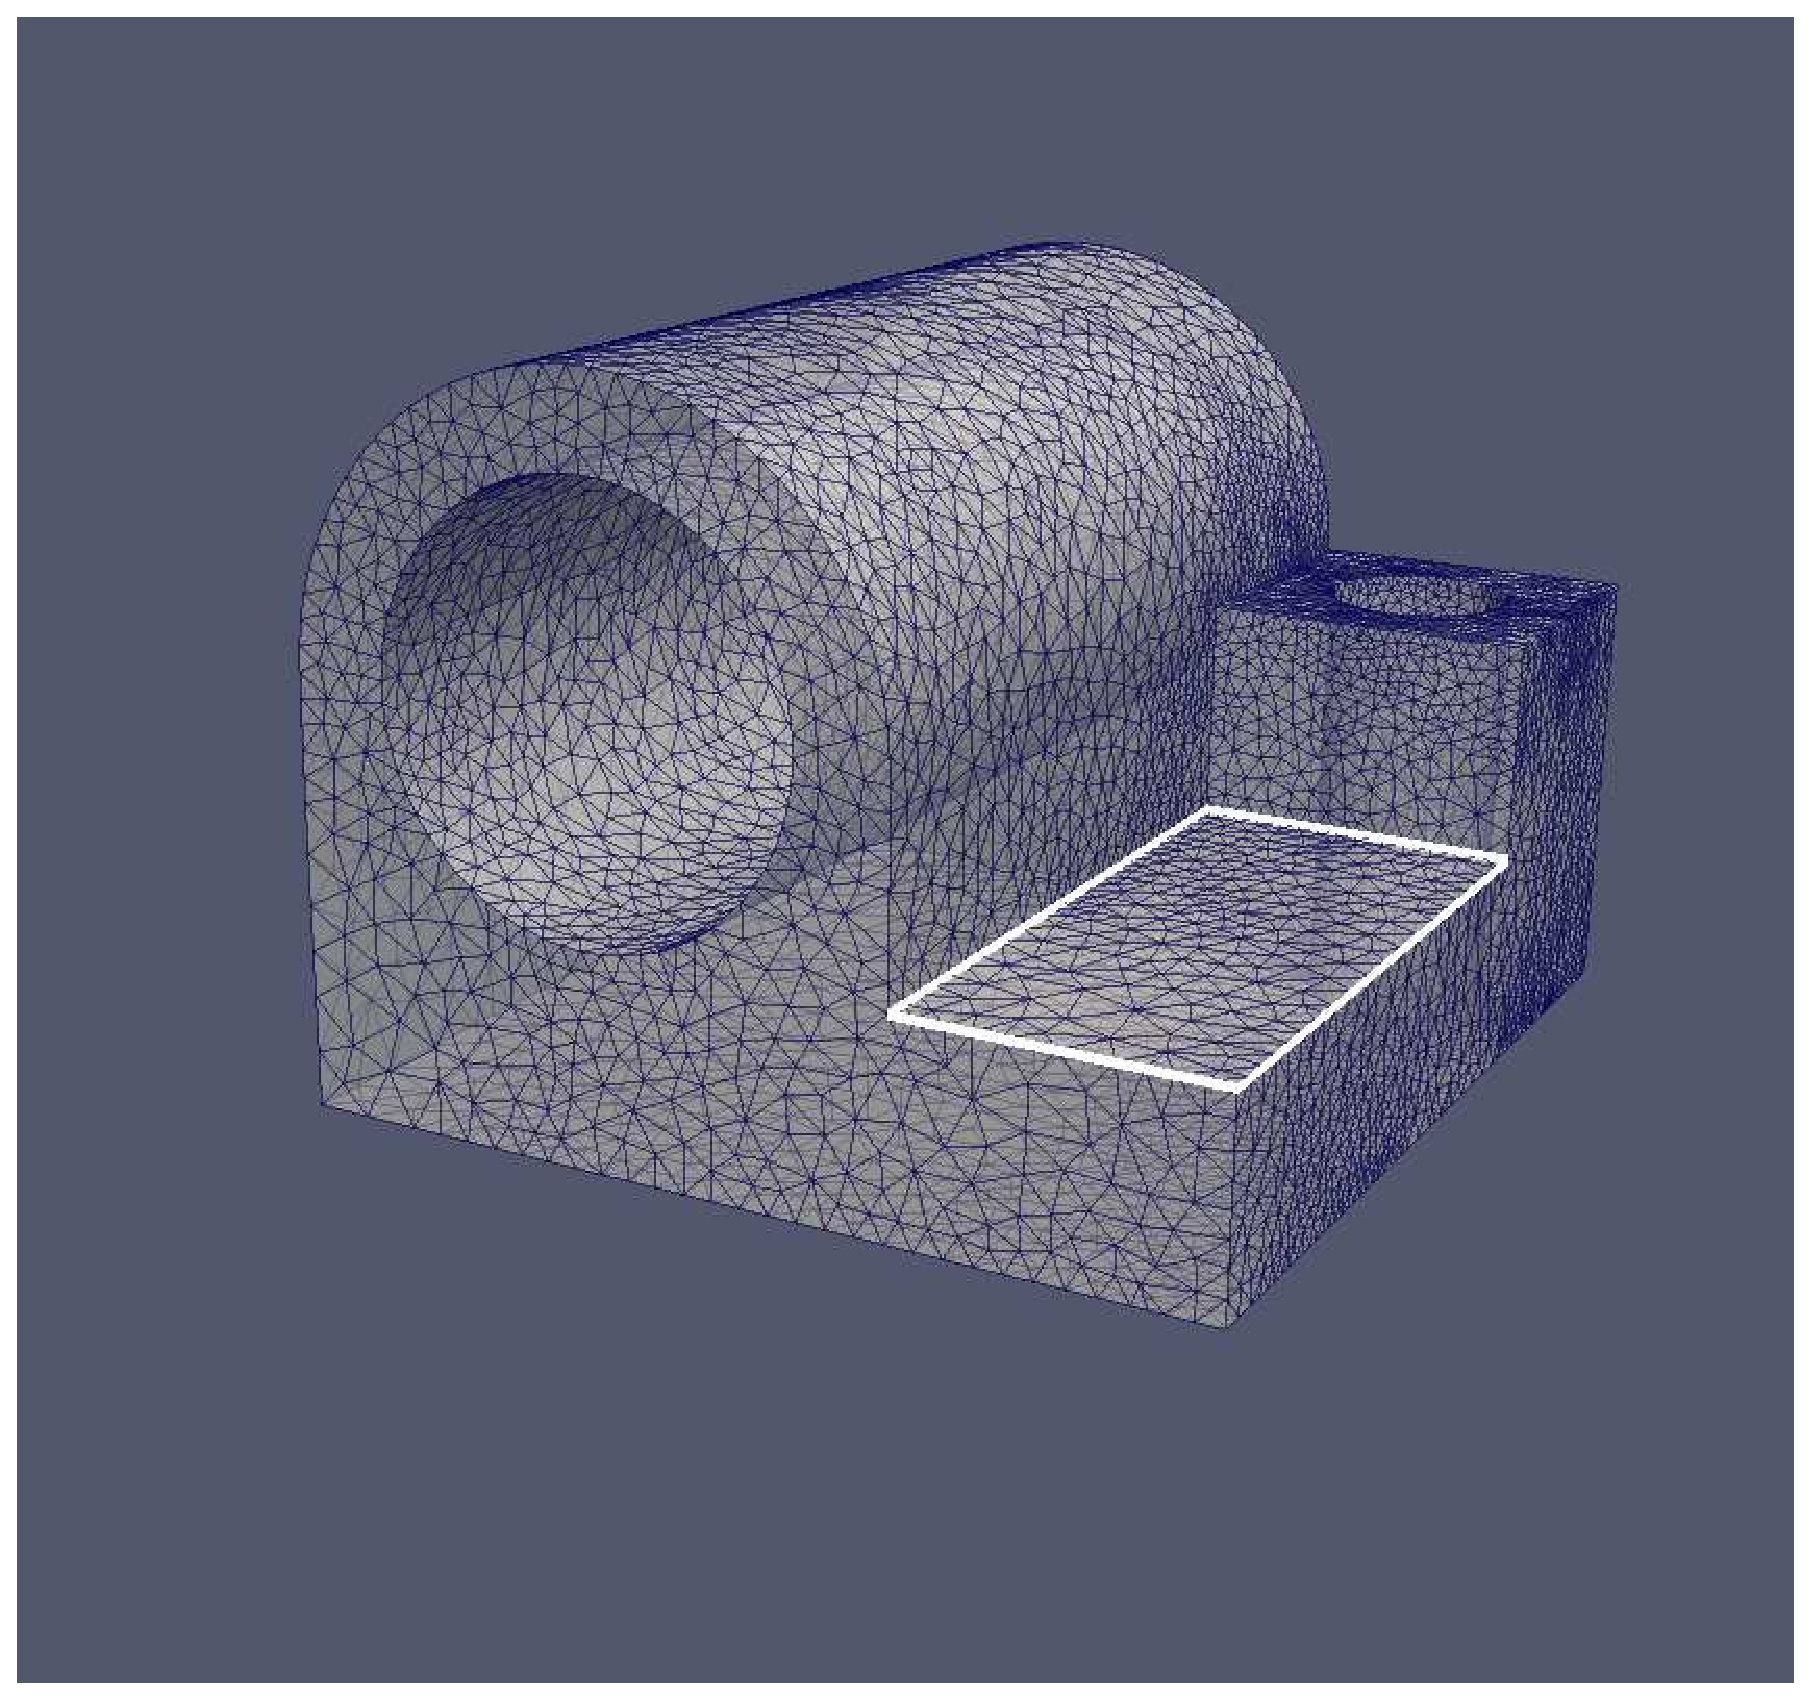
\includegraphics[width=.8\linewidth]{img/m1/surfSegmentation/surf7.eps}
  \caption{}
  \label{surf3}
\end{subfigure}
\caption{An example input triangulation of an arbitrary mechanical part. Four of the segmented surfaces are outlined.}
\label{fig-surfSegment}
\end{figure}

\subsection{Advancing Layer Initialization}

Sharp features of the imported surface are used by CGM to segment the surface. The boundary curves of the segmented surface denote these sharp features. For the purpose of this thesis, we consider these identified boundary curves as the initial front of the mesh. In other words, the boundary curves of the segmented surfaces (or sub-surfaces) serve as the zeroth layer of the advancing layer surface mesh.

Picking the boundary curves of the sub-surfaces to serve as the initial front helps us create anisotropy normal to these boundary curves. This way, desired refinement can be obtained normal to these boundary curves, which is a desirable feature as these boundary curves define the surface features. The discretization of the boundary curves imported along with the surface triangulation defines the refinement and gradation along the boundary curves (or along the zeroth front). Hence, the refinement and gradation along the boundary curves of the surface is defined by the input triangulation and is up to the user to vary. The surface mesh generated by EDAM-S hence provides with anisotropy along the normal direction (on the surface) to these boundary curves of the sub-surfaces.

We chose the boundary curves identified by CGM to serve as the zeroth layer of EDAM-S. However,the initial front could be chosen to be something else without affecting the rest of the mesh generation procedure. For eg. curves along high principal curvature directions on the surface could be added to the zeroth layer of the mesh to get the required anisotropy along highly curved regions of the surface. This is a work in progress and might be added to EDAM-S in the future.

\section{Point Placement}

After importing the surface triangulation, we have a valid underlying surface representation with us. Also, segmented sub-surfaces and their boundaries curves provide us with the boundaries we need to march off of. The mesh generation routine starts by initializing the boundaries of each sub-surface of the surface by marking each point on the boundary as a candidate marching point which form the starting layer in the mesh. The points at the boundary curves of the sub-surfaces serve as the parent points for the first layer inserted into the mesh.

The data structure created to store a vertex on the advancing front of the mesh also stores the edges adjacent to that vertex so as to identify the marching directions. Hence, the extrusion direction or marching direction of a point is obtained from the location of the vertex, its adjacent edges, and the underlying sub-surface which is being meshed. The 
to  which is explained in detail in the next subsection. Each edge stores the direction into the interior of the sub-surface it bounds with respect to the surface normal. As the sub-segments sharing a common boundary are meshed independently, it is easy to identify the normal to an edge along the sub-surface for advancing the front in the mesh generation algorithm.

%\begin{lstlisting}[language=cpp,caption={Caption}, frame=bt, numbers=none]
%// Class defining a vertex on the advancing layer
%class edamSurfVert {
%public:
%  int index;  
%  
%}
%\end{lstlisting}

\subsection{Advancing Layer Routine- Point placement} \label{advancing-layer}

For each of the sub-surfaces of the geometry, the advancing layer routine iteratively picks a point from its boundary and extrudes it in a given direction. After evaluating the extruded point, we project the point onto the underlying surface. This process is set up to be of two steps for simplicity, accuracy and computational efficiency as will be explained later.

\begin{figure}
\centering
\begin{subfigure}{0.5\textwidth}
  \centering
  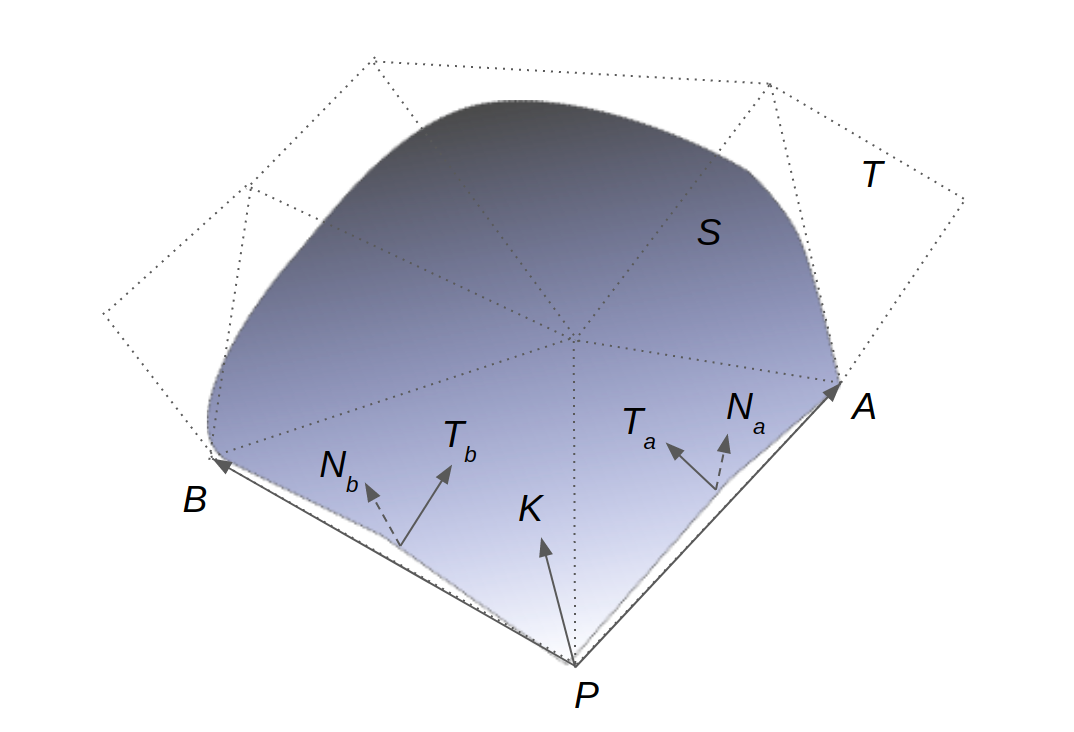
\includegraphics[trim={2cm 0 2cm 0},clip,width=\linewidth]{img/m1/pointPlacement.png}
  \caption{}
  \label{fig-pointPlacement1}
\end{subfigure}%
\begin{subfigure}{0.5\textwidth}
  \centering
  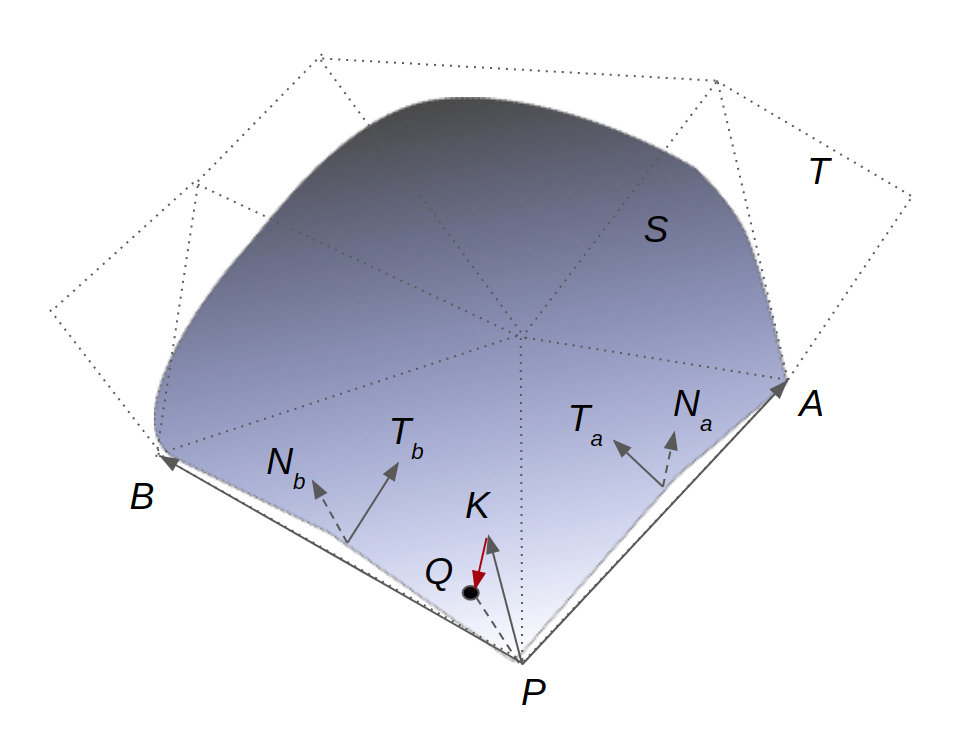
\includegraphics[width=\linewidth]{img/m1/pointProjection.png}
  \caption{}
  \label{fig-pointPlacement2}
\end{subfigure}
\begin{subfigure}{0.5\textwidth}
	\centering
	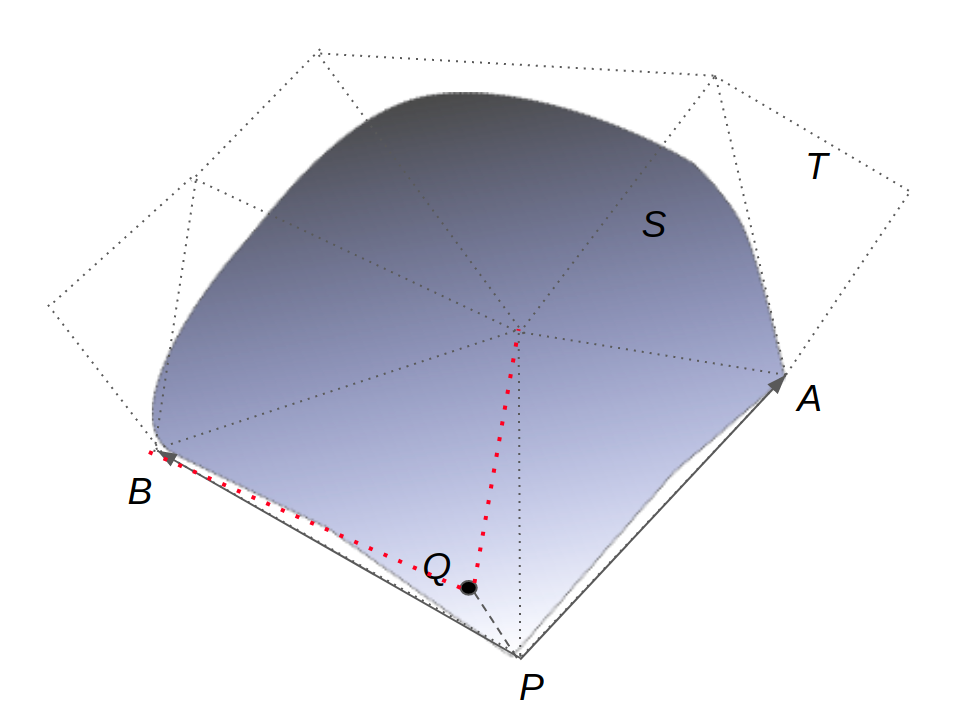
\includegraphics[width=\linewidth]{img/m1/pointInsertion.png}
	\caption{}
	\label{fig-pointPlacement3}
\end{subfigure}%
\begin{subfigure}{0.5\textwidth}
	\centering
	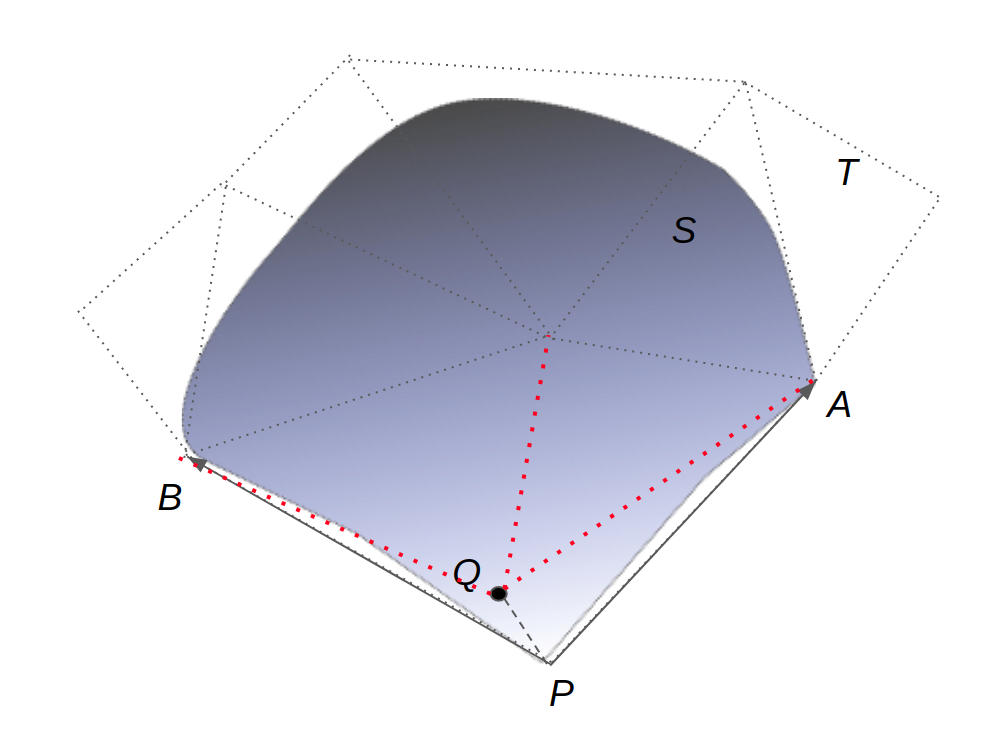
\includegraphics[width=\linewidth]{img/m1/localReconnection.png}
	\caption{}
	\label{fig-pointPlacement4}
\end{subfigure}
\caption{}
\label{fig-point}
\end{figure}

In the first step, we extrude the parent point to get the extruded point. We would interchangeably call the extruded points as the kid points as they represent the successors of their parent points from the previous layer. The direction of this extrusion is set up to be the average of the normals of the parent vertex's adjacent edges in the tangential plane of the sub-surface. In other words, the normals of the adjacent two edges of a vertex on the underlying sub-surface are averaged to get the extrusion direction.

Consider Figure \ref{fig-point}. Initial input triangulation is marked $T$ and the bezier surface representation is marked $S$. Point $P$ is at the boundary curve of the surface. We need to find the extrusion direction of P to know where its kid would be located. In the underlying triangulation $T$, $PB$ and $PA$ are the edges adjacent to $P$ on the boundary of the surface $S$. We first find the mid-points of quartic-Bezier curves $PB$ and $PA$ which are constructed by CGM as a part of constructing the quartic-Bezier triangular surface patches from the underlying triangulation $T$. Next, we find the normal directions on the surface at these mid-points. The normal directions are carefully queried from the sub-surface which is being meshed currently. The normal directions are labeled as $N_b$ and $N_a$ in the figure. We cross product the vector $PB$ with $N_b$ to get the direction $T_b$. The vector $T_b$ is normal to the edge $PB$ as well as tangential to the surface $S$. Similarly, we find the vector $T_a$. The direction of extrusion $\vec{PK}$ is chosen to be the average of the direction of $T_a$ and $T_b$.

The initial extrusion length is an input parameter provided by the user. This length would be taken as the extrusion length when the boundary points are extruded for the first time to the interior of the surface. This length can vary with boundary vertices as the points are extruded independently. Hence, this extrude length can either be supplied by the user for all the points of the boundary separately or as a single value for all the boundary points. To obtain best quality quad elements, we scale the extrusion length at a given vertex on the advancing layer with respect to the interior angle between the direction vectors $T_a$ and $T_b$. If the vertex is a concave corner vertex, the extrusion length is increased so as to create good quality quad elements in the next layer. This process is described in detail in section \ref{section-extrusionScaling}.%and vice-versa for convex corner vertices. Also, if the vertex is a convex corner, additional marching directions are added so as to sufficiently refine the interior domain of the surface. The number of additional marching directions added depends on the convexity of the vertex. If we have $n$ marching directions for a point, the angle between the adjacent edges would be divided into $n+1$ angles to get the marching directions for the $n$ points. We hope to include these modifications in the final paper submission.

After we have extruded the point, we project it on to the underlying geometry. This operation ensures that all the  points we insert in the mesh are on the underlying geometry. Errors here would compound in subsequent layers. Points are inserted in the mesh and the mesh elements are subdivided to include the new point. The candidate point for insertion can subdivide an existing triangle to replace the previous triangle with three new ones, or can subdivide an edge to replace existing two triangles with four new ones. To find the best triangle or edge for subdivision, we first make a guess for the triangle to insert the point. Any triangle in the surface interior adjacent to the point being extruded is chosen. Starting from this triangle, we iteratively jump to the best edge or triangle by comparing the barycentric coordinates of the new point with respect to the triangle in consideration. This technique suffers from two disadvantages. First, we need to compare double precision values of barycentric coordinates for making a decision on which triangle to choose for insertion. If the values are too close, the point might be inserted in the wrong triangle and would eventually lead to deviation of the mesh from the underlying surface. Second, the process of iteratively finding the right triangle for insertion might end up being in an infinite loop. Both of these problems are substantially reduced with a good isotropic initial triangulation. However, we add several validity tests to avoid these problems even for a coarse initial triangulation. These include orientation checks of the triangles formed with respect to the surface, thresholding the maximum deviation of the newly formed triangle from the surface and thresholding the dihedral angles between two triangles on the surface. We use an epsilon value of $10^{-5}$ while comparing the values of barycentric coordinates to zero. Also, we insert the point on a face rather than in a triangle when the ratio of the second-smallest barycentric coordinate to the smallest one is more than a set threshold ($10^2$). This helps us avoid very skinny triangles with large obtuse angles and also helps in avoiding several unnecessary face swapping in the mesh.

After advancing one layer to the surface interior, we increase the extrude length at each point by a factor. This factor, called the growth ratio, specifies the anisotropic layer-on-layer extrusion length growth as we march on the surface. A value of growth ratio between 1.1 and 1.4 gives us satisfactory anisotropy at the boundaries of the mesh.

%\begin{figure}
%    \centering
%    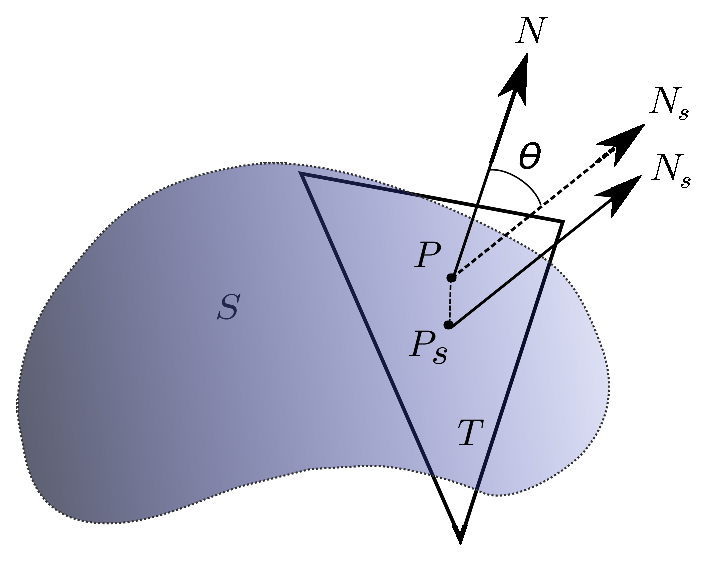
\includegraphics[width=.3\textwidth]{deviate-surface.eps}
%    \caption{Triangle $T$ deviates from the underlying surface $S$. $P$ is the centroid of $T$ and $P_s$ is the projection of $P$ on $S$. The deviation is calculated as the interior angle between the normal to the triangle $PN$ and the normal to the surface at $P_s$, which is $P_sN_s$. The angle $\theta$ represents the deviation here. The deviation is exaggerated for illustration purposes.}
%    \label{deviation-surface}
%\end{figure}

\section{Local Reconnection for quality}


